\documentclass[11pt]{article}
\usepackage[utf8]{inputenc}
\usepackage[dvips]{graphicx}
\usepackage{graphicx}
\usepackage{fancybox}
\usepackage{verbatim}
\usepackage{array}
\usepackage{latexsym}
\usepackage{alltt}
\usepackage{hyperref}
\usepackage{textcomp}
\usepackage{color}
\usepackage{amsmath}
\usepackage{amsfonts}
\usepackage{tikz}
\usepackage{float}
\usepackage{pdfpages}
\usepackage[most]{tcolorbox}
\usepackage{multicol}
\usepackage[hmargin=3cm,vmargin=5.0cm]{geometry}
%\topmargin=0cm
\topmargin=-2cm
\addtolength{\textheight}{6.5cm}
\addtolength{\textwidth}{2.0cm}
%\setlength{\leftmargin}{-5cm}
\setlength{\oddsidemargin}{0.0cm}
\setlength{\evensidemargin}{0.0cm}

\geometry
{
 a4paper,
 left=15mm,
 top=15mm,
}

\newtcolorbox{mybox}[3][breakable]
{
  colframe = #2!25,
  colback  = #2!10,
  coltitle = #2!20!black,  
  title    = {#3},
  #1,
}

\newenvironment{example}[1][\unskip]{\begin{mybox}{green}{\textbf{Example} {#1}}}{\end{mybox}}
\newenvironment{definition}[1]{\begin{mybox}{blue}{\textbf{Definition #1}}}{\end{mybox}}
\newenvironment{theorem}[1]{\begin{mybox}{red}{\textbf{Theorem #1}}}{\end{mybox}}


\title{CENG 223 - Chapter 8: Advanced Counting Techniques}
\author{Burak Metehan Tunçel}
\date{January 2022}

\begin{document}

\maketitle
\section{Applications of Recurrence Relations}

\subsection{Introduction}

A \textbf{recurrence relation} is an equation that defines a sequence based on a rule that gives the next term as a function of the previous term(s).

The simplest form of a recurrence relation is the case where the next term depends only on the immediately previous term. If we denote the $n^{th}$ term in the sequence by $x_n$, such a recurrence relation is of the form

\begin{equation*}
    x_{n+1} = f(x_n)
\end{equation*}


\subsection{Modeling With Recurrence Relations}

We can use \textit{recurrence relations to model a wide variety of problems}, such as finding compound interest, counting rabbits on an island, determining the number of moves in the Tower of Hanoi puzzle, and counting bit strings with certain properties.

\begin{example}
%\begin{tcolorbox}[breakable]
%\textbf{Example}

Find a recurrence relation and give initial conditions for the number of bit strings of length $n$ that do not have two consecutive $0$s. How many such bit strings are there of length five?\\

\textbf{Solution}

Let $a_n$ denote the number of bit strings of length $n$ that do not have two consecutive $0$s. We assume that $n \geq 3$, so that the bit string has at least three bits. Strings of this sort of length $n$ can be divided into those that end in $1$ and those that end in $0$. The bit strings of length $n$ ending with $1$ that do not have two consecutive $0$s are precisely the bit strings of length $n - 1$ with no two consecutive $0$s with a $1$ added at the end. Consequently, there are $a_n - 1$ such bit strings.

Bit strings of length $n$ ending with a $0$ that do not have two consecutive $0$s must have
$1$ as their $(n - 1)^{st}$ bit; otherwise they would end with a pair of $0$s. Hence, the bit strings of length $n$ ending with a $0$ that have no two consecutive $0$s are precisely the bit strings of length $n - 2$ with no two consecutive $0$s with $10$ added at the end. Consequently, there are $a_n - 2$ such bit strings.


We conclude, as illustrated in Figure 1, that

\begin{align*}
    &a_n = a_{n - 1} + a_{n - 2} &\text{for } n \geq 3    
\end{align*}

The initial conditions are $a_1 = 2$, because both bit strings of length one, $0$ and $1$ do not have consecutive $0$s, and $a_2 = 3$, because the valid bit strings of length two are $01$, $10$, and $11$. To obtain $a_5$, we use the recurrence relation three times to find that

\begin{align*}
    &a_3 = a_2 + a_1 = 3 + 2 = 5\\
    &a_4 = a_3 + a_2 = 5 + 3 = 8\\
    &a_5 = a_4 + a_3 = 8 + 5 = 13
\end{align*}

\textbf{Remark:} Note that \{$a_n$\} satisfies the same recurrence relation as the Fibonacci sequence. Because $a_1 = f_3$ and $a_2 = f_4$ it follows that $a_n = f_{n+2}$.
%\end{tcolorbox}
\end{example}

\begin{figure}[h]
    \centering
    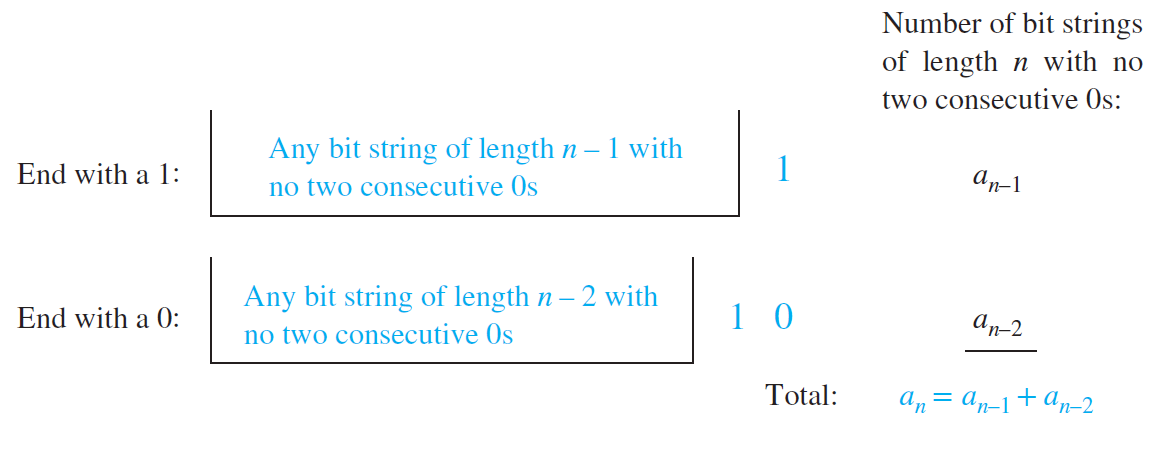
\includegraphics[width=0.5\textwidth]{bit-string.png}
    \caption{Counting bit strings of length n with no two consecutive $0$s.}
    \label{fig:my_label}
\end{figure}


\section{Solving Linear Recurrence Relations}

\subsection{Introduction}

\begin{definition}
{1}
A \textit{linear homogeneous recurrence relation of degree k with constant coefficients} is a recurrence relation of the form
\begin{equation*}
a_n = c_1a_{n-1} + c_2a_{n-2} + ... + c_ka_{n-k},
\end{equation*}
where $c_1$, $c_2$, ..., $c_k$ are real numbers, and $c_k \neq 0$.
\end{definition}

The recurrence relation in the definition is \textbf{linear} because the \textit{right-hand side is a sum of previous terms} of the sequence each multiplied by a function of $n$. 
The recurrence relation is \textbf{homogeneous} because \textit{no terms occur that are not multiples of the $a_js$}. 
The coefficients of the terms of the sequence are all \textbf{constants}, rather than functions that depend on $n$. 
The \textbf{degree} is $k$ because $a_n$ is expressed in terms of the previous $k$ terms of the sequence.

A consequence of the second principle of mathematical induction is that a sequence satisfying the recurrence relation in the definition is uniquely determined by this recurrence relation and the $k$ initial conditions
\begin{equation*}
    a_0 = C_0, a_1 = C_1, ..., a_{k-1} = C_{k-1}.
\end{equation*}


\begin{example}
The recurrence relation $P_n = (1.11) P_{n-1}$ is a linear homogeneous recurrence relation of degree one. The recurrence relation $f_n = f_{n-1} + f_{n-2}$ is a linear homogeneous recurrence relation of degree two. The recurrence relation $a_n = a_{n-5}$ is a linear homogeneous recurrence relation of degree five. 
\end{example}

To help clarify the definition of linear homogeneous recurrence relations with constant coefficients, we will now provide examples of recurrence relations each lacking one of the defining properties.

\begin{example}
The recurrence relation $a_n = a_{n-1} + a^2_{n-2}$ is not linear. The recurrence relation $H_n = 2H_{n-1} + 1$ is not homogeneous. The recurrence relation $B_n = nB_{n-1}$ does not have constant coefficients. 
\end{example}

Linear homogeneous recurrence relations are studied for two reasons. First, \textit{they often occur in modeling of problems}. Second, \textit{they can be systematically solved}.


\subsection{Solving Linear Homogeneous Recurrence Relations with Constant Coefficients}

Recurrence relations may be difficult to solve, but fortunately this is not the case for \textit{linear homogenous recurrence relations with constant coefficients}. We can use two key ideas to find all their solutions. 
First, \textit{these recurrence relations have solutions of the form $a_n = r^n$}, where
$r$ is a constant. To see this, observe that $a_n = r^n$ is a solution of the recurrence relation $a_n = c_1a_{n-1} + c_2a_{n-2} + ... + c_ka_{n-k}$ if and only if
\begin{equation*}
    r_n = c_1r^{n-1} + c_2r^{n-2} + ... + c_kr^{n-k}
\end{equation*}
When both sides of this equation are divided by $r^{n-k}$ (when $r \neq 0$) and the right-hand side is subtracted from the left, we obtain the equation
\begin{equation*}
    r^k - c_1r^{k-1} - c_2r^{k-2} - ... - c_{k-1}r - c_k = 0.
\end{equation*}

Consequently, the sequence ${a_n}$ with $a_n = r^n$ where $r \neq 0$ is a solution if and only if $r$ is a solution of this last equation. We call this the \textbf{characteristic equation} of the recurrence relation. The solutions of this equation are called the \textbf{characteristic roots} of the recurrence relation. As we will see, these \textit{characteristic roots can be used to give an explicit formula for all the solutions of the recurrence relation}.


The other key observation is that a linear combination of two solutions of a linear homogeneous recurrence relation is also a solution. To see this, suppose that $s_n$ and $t_n$ are both solutions of $a_n = c_1a_{n-1} + c_2a_{n-2} + ... + c_ka_{n-k}$. Then
\begin{equation*}
    s_n = c_1s_{n-1} + c_2s_{n-2} + ... + c_ks_{n-k}    
\end{equation*}
and
\begin{equation*}
    t_n = c_1t_{n-1} + c_2t_{n-2} + ... + c_kt_{n-k}.    
\end{equation*}
Now suppose that $b_1$ and $b_2$ are real numbers. Then
\begin{align*}
    b_1s_n + b_2t_n &= b_1(c_1s_{n-1} + c_2s_{n-2} + ... + c_ks_{n-k}) + b_2(c_1t_{n-1} + c_2t_{n-2} + ... + c_kt_{n-k})\\
    &= c_1(b_1s_{n-1} + b_2t_{n-1}) + c_2(b_1s_{n-2} + b_2t_{n-2}) + ... + c_k(b_1s_{n-k} + b_kt_{n-k}).    
\end{align*}
This means that $b_1s_n + b_2t_n$ is also a solution of the same linear homogeneous recurrence relation.

Using these key observations, we will show how to solve linear homogeneous recurrence
relations with constant coefficients.

\subsubsection{The Degree Two Case}

We now turn our attention to linear homogeneous recurrence relations of degree two. First, consider the case when \textit{there are two distinct characteristic roots}.

\begin{theorem}{1}
Let $c_1$ and $c_2$ be real numbers. Suppose that $r^2 - c_1r - c_2 = 0$ has two distinct roots $r_1$ and $r_2$. Then the sequence ${a_n}$ is a solution of the recurrence relation $a_n = c_1a_{n-1} + c_2a_{n-2}$ if and only if $a_n = \alpha_1r^n_1 + \alpha_2r^n_2$ for $n = 0, 1, 2, ...,$ where $\alpha_1$ and $\alpha_2$ are constants.
\end{theorem}

\textbf{\textit{Proof:}} We must do two things to prove the theorem.\\
First, it must be shown that if $r_1$ and $r_2$ are the roots of the \textit{characteristic equation}, and $\alpha_1$ and $\alpha_2$ are constants, then the sequence ${a_n}$ with $a_n = \alpha_1r^n_1 + \alpha_2r^n_2$ is a solution of the recurrence relation.\\
Second, it must be shown that if the sequence ${a_n}$ is a solution, then $a_n = \alpha_1r^n_1 + \alpha_2r^n_2$ for some constants $\alpha_1$ and $\alpha_2$

We now show that if $a_n = \alpha_1r^n_1 + \alpha_2r^n_2$, then the sequence $\{a_n\}$ is a solution of the recurrence relation. Because $r_1$ and $r_2$ are roots of $r^2 - c_1r - c_2 = 0$, it follows that $r^2_1 = c_1r_1 + c_2$ and $r^2_2 = c_1r_2 + c_2$.

From these equations, we see that

\begin{align*}
    c_1a_{n-1} + c_2a_{n-2} &= c_1(\alpha_1r^{n-1}_1 + \alpha_2r^{n-1}_2) + c_2(\alpha_1r_1^{n-2} + \alpha_2r_2^{n-2})\\
    &= \alpha_1r^{n-2}_1(c_1r_1 + c_2) + \alpha_2r^{n-2}_2(c_1r_2 + c_2)\\
    &= \alpha_1r^{n-2}_1r_1^2 + \alpha_2r^{n-2}_2r_2^2\\
    &= \alpha_1r^n_1 + \alpha_2r^n_2\\
    &= a_n
\end{align*}

\textit{(Proof continues. It should be read from textbook, page 542)}.\\

The characteristic roots of a linear homogeneous recurrence relation with constant coefficients may be complex numbers. Theorem 1 (and also subsequent theorems in this section) still applies in this case. Recurrence relations with complex characteristic roots will not be discussed in the text. \\

Theorem 1 does not apply when there is one characteristic root of multiplicity two. If this happens, then $a_n = nr^n_0$ is another solution of the recurrence relation when $r_0$ is a root of multiplicity two of the characteristic equation. Theorem 2 shows how to handle this case.

\begin{theorem}{2}
Let $c_1$ and $c_2$ be real numbers with $c_2 \neq 0$. Suppose that $r^2 - c_1 r - c_2 = 0$ has only one root $r_0$. A sequence $\{a_n\}$ is a solution of the recurrence relation $a_n = c_1a_{n-1} + c_2a_{n-2}$ if and only if $a_n = \alpha_1 r^n_0 + \alpha_2 nr^n_0$, for $n = 0, 1, 2, ...$, where $\alpha_1$ and $\alpha_2$ are constants.
\end{theorem}

\subsubsection{The General Case}

We will now state the general result about the solution of linear homogeneous recurrence relations with constant coefficients, where the degree may be greater than two, under the assumption that the characteristic equation has distinct roots.

\begin{theorem}{3}
Let $c_1, c_2, ..., c_k$ be real numbers. Suppose that he characteristic equation
\begin{equation*}
    r^k - c_1r^{k-1} - \cdot \cdot \cdot - c_k = 0
\end{equation*}
has $k$ distinct roots $r_q, r_2, ..., r_k$. Then a sequence $\{a_n\}$ is a solution of the recurrence relation
\begin{equation*}
    a_n = c_1a_{n-1} + c_2a_{n-2} + \cdot \cdot \cdot + c_ka_{n-k}
\end{equation*}
if and only if
\begin{equation*}
    a_n = \alpha_1r_1^n + \alpha_2r_2^n + \cdot \cdot \cdot + \alpha_kr_k^n
\end{equation*}
for $n = 0, 1, 2, ...$ where $\alpha_1, \alpha_2, ..., \alpha_k$ are constants.
\end{theorem}

We now state the most general result about linear homogeneous recurrence relations with constant coefficients, allowing the characteristic equation to have multiple roots. The key point is that for each root $r$ of the characteristic equation, the general solution has a summand of the form $P(n)r^n$, where $P(n)$ is a polynomial of degree $m - 1$, with $m$ the multiplicity of this root.

\begin{theorem}{4}
Let $c_1, c_2, ..., c_k$ be real numbers. Suppose that the characteristic equation
\begin{equation*}
    r^k - c_1r^{k-1} - \cdot \cdot \cdot - c_k = 0
\end{equation*}

has $t$ distinct roots $r_1, r_2, ..., r_t$ with multiplicities $m_1, m_2, ..., m_t$, respectively, so that $m_i \geq 1$ for $i = 1, 2, ..., t$ and $m_1 + m_2 + \cdot \cdot \cdot + m_t = k$. Then a sequence $\{a_n\}$ is a solution of the recurrence relation
\begin{equation*}
    a_n = c_1a_{n-1} + c_2a_{n-2} + \cdot \cdot \cdot + c_ka_{n-k}
\end{equation*}
if and only if
\begin{align*}
    a_n =\ &(\alpha_{1,0} + \alpha_{1,1}n + \cdot \cdot \cdot + \alpha_{1,m_1-1}n^{m_1-1})r_1^n \\
    &+ (\alpha_{2,0} + \alpha_{2,1}n + \cdot \cdot \cdot + \alpha_{2,m_2-1}n^{m_2-1})r_2^n\\
    &+ \cdot \cdot \cdot + (\alpha_{t,0} + \alpha_{t,1}n + \cdot \cdot \cdot + \alpha_{t,m_t-1}n^{m_t-1})r_t^n
\end{align*}
for $n = 0, 1, 2, ...$, where $\alpha_{i,j}$ are constants for $1 \leq i \leq t$ and $0 \leq j \leq m_i - 1$.
\end{theorem}

\begin{example}
Suppose that the roots of the characteristic equation of a linear homogeneous recurrence relation are 2, 2, 2, 5, 5, and 9 (that is, there are three roots, the root 2 with multiplicity three, the root 5 with multiplicity two, and the root 9 with multiplicity one). What is the form of the general solution?

\textbf{Solution:} By Theorem 4, the general form of the solution is
\begin{equation*}
    (\alpha_{1,0} + \alpha_{1,1}n + \alpha_{1,2}n^2)2^n + (\alpha_{2,0} + \alpha_{2,1}n)5^n + \alpha_{3,0}9^n
\end{equation*}
\end{example}

\subsection{Linear Nonhomogeneous Recurrence Relations with Constant Coefficients}

We have seen how to solve linear homogeneous recurrence relations with constant coefficients. Is there a relatively simple technique for solving a linear, but not homogeneous, recurrence relation with constant coefficients, such as $a_n = 3a_{n-1} + 2n$? We will see that the answer is yes for certain families of such recurrence relations.

The recurrence relation $a_n = 3a_{n-1} + 2n$ is an example of a \textbf{linear nonhomogeneous recurrence relation with constant coefficients}, that is, a recurrence relation of the form

$a_n = c_1a_{n-1} + c_2a_{n-2} + \cdot \cdot \cdot + c_ka_{n-k} + F(n)$

where $c_1, c_2, ..., c_k$ are real numbers and $F(n)$ is a function not identically zero depending only on $n$. The recurrence relation

$a_n = c_1a_{n-1} + c_2a_{n-2} + \cdot \cdot \cdot + c_ka_{n-k}$

is called the \textbf{associated homogeneous recurrence relation}. It plays an important role in the solution of the nonhomogeneous recurrence relation.

The key fact about linear nonhomogeneous recurrence relations with constant coefficients is that \textit{every solution is the sum of a particular solution and a solution of the associated linear homogeneous recurrence relation}, as Theorem 5 shows

\begin{theorem}
{5}
If $\{a_n^{(p)}\}$ is a particular solution of the nonhomogeneous linear recurrence relation with constant coefficients
\begin{align*}
    a_n = c_1a_{n-1} + c_2a_{n-2} + \cdot \cdot \cdot + c_ka_{n-k} + F(n) & & & & & & & &  &
\end{align*}
then every solution is of the form $\{a_n^{(p)} + a_n^{(h)}\}$, where $\{a_n^{(h)}\}$ is a solution of the associated homogeneous recurrence relation
\begin{align*}
    a_n = c_1a_{n-1} + c_2a_{n-2} + \cdot \cdot \cdot + c_ka_{n-k} & & & & & & & &  &
\end{align*}
\end{theorem}

\textit{(The proof of the Theorem 5 should be read from the textbook)}.

By Theorem 5, we see that the key to solving nonhomogeneous recurrence relations with constant coefficients is finding a particular solution. Then every solution is a sum of this solution and a solution of the associated homogeneous recurrence relation. Although there is no general method for finding such a solution that works for every function $F(n)$, there are techniques that work for certain types of functions $F(n)$, such as polynomials and powers of constants.

\begin{example}
Find all solutions of the recurrence relation $a_n = 3a_{n-1} + 2n$. What is the solution with $a_1 = 3$?

\textbf{Solution:}
To solve this linear nonhomogeneous recurrence relation with constant coefficients, we need to solve its associated linear homogeneous equation and to find a particular solution for the given nonhomogeneous equation. The associated linear homogeneous equation is $a_n = 3a_{n-1}$. Its solutions are $a_n^{(h)} = \alpha 3^n$, where $\alpha$ is a constant.\\

We now find a particular solution. Because $F(n) = 2n$ is a polynomial in $n$ of degree one, a reasonable trial solution is a linear function in $n$, say, $p_n = cn + d$, where $c$ and $d$ are constants. To determine whether there are any solutions of this form, suppose that $p_n = cn + d$ is such a solution. Then the equation $a_n = 3a_{n-1} + 2n$ becomes $cn + d = 3(c(n - 1) + d) + 2n$. Simplifying and combining like terms gives $(2 + 2c)n+ (2d - 3c) = 0$. It follows that $cn + d$ is a solution if and only if $2 + 2c = 0$ and $2d - 3c = 0$. This shows that $cn + d$ is a solution if and only if $c = -1$ and $d = -3/2$. Consequently, $a_n^{(p)} = -n - 3/2$ is a particular solution.\\

By Theorem 5 all solutions are of the form
\begin{align*}
    a_n = a_n^{(p)} + a_n^{(h)} = -n - \frac{3}{2} + \alpha \cdot 3^n & & & & & & & &  &
\end{align*}
where $\alpha$ is a constant.\\

To find the solution with $a_1 = 3$, let $n = 1$ in the formula we obtained for the general solution. We find that $3 = -1 - 3/2 + 3\alpha$, which implies that $\alpha = 11/6$. The solution we seek is $a_n = -n - 3/2 + (11/6)3^n$
\end{example}

\begin{example}
Find all solutions of the recurrence relation
\begin{align*}
    a_n = 5a_{n-1} - 6_{n-2} + 7^n & & & & & & & & &
\end{align*}

\textbf{Solution:} 
This is a linear nonhomogeneous recurrence relation. The solutions of its associated homogeneous recurrence relation
\begin{align*}
   a_n = 5a_{n-1} - 6a_{n-2} & & & & & & & & & 
\end{align*}

are $a_n^{(h)} = \alpha_1 \cdot 3^n + \alpha_2 \cdot 2^n$, where $\alpha_1$ and $\alpha_2$ are constants. Because $F(n) = 7^n$, a reasonable trial solution is $a_n^{(p)} = C \cdot 7^n$, where $C$ is a constant. Substituting the terms of this sequence into the recurrence relation implies that $C \cdot 7^n = 5C \cdot 7^{n-1} - 6C \cdot 7^{n-2} + 7^n$. Factoring out $7^{n-2}$, this equation becomes $49C = 35C - 6C + 49$, which implies that $20C = 49$, or that $C = 49/20$.
Hence, $a_n^{(p)} = (49/20)7^n$ is a particular solution. By Theorem 5, all solutions are of the form
\begin{align*}
    a_n = \alpha_1 \cdot 3^n + \alpha_2 \cdot 2^n + (49/20)7^n & & & & & & & & &
\end{align*}
\end{example}

\newpage In above two examples, we made an educated guess that there are solutions of a particular form. In both cases, we were able to find particular solutions. This was not an accident. \textit{Whenever $F(n)$ is the product of a polynomial in $n$ and the $n$th power of a constant, we know exactly what form a particular solution has}, as stated in Theorem 6.

\begin{theorem}{6}
Suppose that $\{a_n\}$ satisfies the linear nonhomogeneous recurrence relation
\begin{align*}
    a_n = c_1a_{n-1} + c_2a_{n-2} + \cdot \cdot \cdot + c_ka_{n-k} + F(n) & & & & & & & & &
\end{align*}
where $c_1, c_2, ..., c_k$ are real numbers, and 
\begin{align*}
    F(n) = (b_tn^t + b_{t-1}n^{t-1} + \cdot \cdot \cdot + b_1n + b_0)s^n & & & & & & & & &
\end{align*}
where $b_0, b_1, ..., b_t$ and $s$ are real numbers. When $s$ is not a root of the characteristic equation of the associated linear homogeneous recurrence relation, there is a particular solution of the form
\begin{align*}
    (p_tn^t + p_{t-1}n{t-1} + \cdot \cdot \cdot + p_1n + p_0)s^n & & & & & & & & &
\end{align*}
When $s$ is a root of this characteristic equation and its multiplicity is $m$, there is a particular solution of the form
\begin{align*}
    n^m(p_tn^t + p_{t-1}n{t-1} + \cdot \cdot \cdot + p_1n + p_0)s^n & & & & & & & & &
\end{align*}
\end{theorem}

Note that in the case when $s$ is a root of multiplicity $m$ of the characteristic equation of the associated linear homogeneous recurrence relation, the factor $n^m$ ensures that the proposed particular solution will not already be a solution of the associated linear homogeneous recurrence relation. 

\begin{example}
What form does a particular solution of the linear nonhomogeneous recurrence relation $a_n = 6a_{n-1} - 9a_{n-2} + F(n)$ have when $F(n) = 3^n$, $F(n) = n3^n$, $F(n) = n^22^n$, and $F(n) = (n^2 + 1)3^n$?

\textbf{Solution:}
The associated linear homogeneous recurrence relation is $a_n = 6a_{n-1} - 9a_{n-2}$. Its characteristic equation, $r^2 - 6r + 9 = (r - 3)^2 = 0$, has a single root, 3, of multiplicity two. To apply Theorem 6, with $F(n)$ of the form $P(n)s^n$, where $P(n)$ is a polynomial and $s$ is a constant, we need to ask whether $s$ is a root of this characteristic equation.\\

Because $s = 3$ is a root with multiplicity $m = 2$ but $s = 2$ is not a root, Theorem 6 tells us that a particular solution has the form
\begin{itemize}
    \item $p_0n^23^n$ if $F(n) = 3^n$
    \item $n^2(p_1n + p_0)3^n$ if $F(n) = n3^n$
    \item $(p_2n^2 + p_1n + p_0)2^n$ if $F(n) = n^22^n$
    \item $n^2(p_2n^2 + p_1n + p_0)3^n$ if $F(n) = (n^2 + 1)3^n$
\end{itemize}
\end{example}


\section{Divide-and-Conquer Algorithms and Recurrence Relations}

\subsection{Introduction}

In computer science, \textbf{divide and conquer} is an \textit{algorithm design paradigm}. A \textbf{divide-and-conquer algorithm} recursively breaks down a problem into two or more sub-problems of the same or related type, until these become simple enough to be solved directly. The solutions to the sub-problems are then combined to give a solution to the original problem. 

These algorithms are called divide-and-conquer algorithms, because they \textit{divide a problem into one or more instances of the same problem of smaller size} and they \textit{conquer the problem by using the solutions of the smaller problems to find a solution of the original problem}, perhaps with some additional work.

In this section we will show how recurrence relations can be used to analyze the computational complexity of divide-and-conquer algorithms. We will use these recurrence relations to estimate the number of operations used by many different divide-and-conquer algorithms.

\subsection{Divide-and-Conquer Recurrence Relations}

Suppose that a recursive algorithm divides a problem of size $n$ into $a$ subproblems, where each subproblem is of size $n/b$ (for simplicity, assume that $n$ is a multiple of $b$; in reality, the smaller problems are often of size equal to the nearest integers either less than or equal to, or greater than or equal to, $n/b$). Also, suppose that a total of $g(n)$ extra operations are required in the conquer step of the algorithm to combine the solutions of the subproblems into a solution of the original problem. Then, if $f(n)$ represents the number of operations required to solve the problem of size $n$, it follows that $f$ satisfies the recurrence relation

$f(n) = a f(n/b) + g(n)$

\noindent This is called a \textbf{divide-and-conquer recurrence relation}.

We will first set up the divide-and-conquer recurrence relations that can be used to study the complexity of some important algorithms. Then we will show how to use these divide-and-conquer recurrence relations to estimate the complexity of these algorithms.

\begin{example}[Binary Search]
Binary search algorithm reduces the search for an element in a search sequence of size $n$ to the binary search for this element in a search sequence of size $n/2$, when $n$ is even. (Hence, the problem of size $n$ has been reduced to one problem of size $n/2$.) Two comparisons are needed to implement this reduction (one to determine which half of the list to use and the other to determine whether any terms of the list remain). Hence, if $f(n)$ is the number of comparisons required to search for an element in a search sequence of size $n$, then
\begin{align*}
    f(n) = f(n/2) + 2 & & & & & & & & &
\end{align*}
when $n$ is even.
\end{example}

\newpage
\begin{example}[Finding the Maximum and Minimum of a Sequence]
Consider the following algorithm for locating the maximum and minimum elements of a sequence $a_1, a_2, ..., a_n$. If $n = 1$, then $a_1$ is the maximum and the minimum. If $n > 1$, split the sequence into two sequences, either where both have the same number of elements or where one of the sequences has one more element than the other. The problem is reduced to finding the maximum and minimum of each of the two smaller sequences. The solution to the original problem results from the comparison of the separate maxima and minima of the two smaller sequences to obtain the overall maximum and minimum.\\

Let $f(n)$ be the total number of comparisons needed to find the maximum and minimum elements of the sequence with $n$ elements. We have shown that a problem of size $n$ can be reduced into two problems of size $n/2$, when $n$ is even, using two comparisons, one to compare the maxima of the two sequences and the other to compare the minima of the two sequences. This gives the recurrence relation
\begin{align*}
    f(n) = 2f(n/2) + 2 & & & & & & & & &
\end{align*}
when $n$ is even.
\end{example}

\begin{example}[Merge Sort]
The merge sort algorithm splits a list to be sorted with $n$ items, where $n$ is even, into two lists with $n/2$ elements each, and uses fewer than $n$ comparisons to merge the two sorted lists of $n/2$ items each into one sorted list. Consequently, the number of comparisons used by the merge sort to sort a list of $n$ elements is less than $M(n)$, where the function $M(n)$ satisfies the divide-and-conquer recurrence relation
\begin{align*}
    M(n) = 2M(n/2) + n & & & & & & & & &
\end{align*}
\end{example}

As above examples show, recurrence relations of the form $f(n) = af(n/b) + g(n)$ arise in many different situations. It is possible to derive estimates of the size of functions that satisfy such recurrence relations. Suppose that f satisfies this recurrence relation whenever $n$ is divisible by $b$. Let $n = b^k$, where $k$ is a positive integer. Then
\begin{align*}
    f(n) &= af(n/b) + g(n)\\
    &= a^2f(n/b^2) + ag(n/b) + g(n)\\
    &= a^3f(n/b^3) + a^2g(n/b^2) + ag(n/b) + g(n)\\
    &\vdots\\
    &= a^kf(n/b^k) + \sum_{j=0}^{k-1}a^jg(n/b^j)
\end{align*}
Because $n/b^k = 1$, it follows that
\begin{equation*}
    f(n) = a^kf(1) + \sum_{j=0}^{k-1} a^j(n/b^j)
\end{equation*}
We can use this equation for $f(n)$ to estimate the size of functions that satisfy divide-and-conquer relations.

\begin{theorem}
{1}
Let $f$ be an increasing function that satisfies the recurrence relation
\begin{align*}
    f(n) = af(n/b) + c & & & & & & & & &
\end{align*}
whenever $n$ is divisible by $b$, where $a \geq 1$, $b$ is an integer greater than 1, and $c$ is a positive real number. Then
\begin{align*}
    f(n) \text{ is } \begin{cases}
       O(n^{\log_b a}) & \text{if } a > 1\\
       O(\log n) & \text{if } a = 1\\
    \end{cases} & & & & & & & & &
\end{align*}
Furthermore, when $n = b^k$ and $a \neq 1$, where $k$ is a positive integer,
\begin{align*}
    f(n) = C_1 n^{\log_b a} + C_2 & & & & & & & & &
\end{align*}
where $C_1 = f(1) + c/(a - 1)$ and $C_2 = -c/(a - 1)$
\end{theorem}

\textit{(Proof of the Theorem 1 should be read from text book)}.

We can use Theorem 1 to estimate the computational complexity of the binary search algorithm and the algorithm given in example above for locating the minimum and maximum of a sequence.

\begin{example}
Give a big-$O$ estimate for the number of comparisons used by a binary search.

\textbf{Solution:}
It was shown that $f(n) = f(n/2) + 2$ when $n$ is even, where $f$ is the number of comparisons required to perform a binary search on a sequence of size $n$. Hence, from Theorem 1, it follows that $f(n)$ is $O(\log n)$.
\end{example}

\begin{example}
Give a big-$O$ estimate for the number of comparisons used to locate the maximum and minimum elements in a sequence using the algorithm given in above examples.

\textbf{Solution:}
We showed that $f(n) = 2f(n/2) + 2$, when $n$ is even, where $f$ is the number of comparisons needed by this algorithm. Hence, from Theorem 1, it follows that $f(n)$ is $O(n^{\log_2 2}) = O(n)$.
\end{example}

\newpage
We now state a more general, and more complicated, theorem, which has Theorem 1 as a special case. This theorem (or more powerful versions, including big-Theta estimates) is sometimes known as the \textit{master theorem} because it is useful in analyzing the complexity of many important divide-and-conquer algorithms.

\begin{theorem}{2}
\textbf{Master Theorem}\\

Let $f$ be an increasing function that satisfies the recurrence relation
\begin{align*}
    f(n) = af(n/b) + cn^d & & & & & & & & &
\end{align*}
whenever $n = b^k$, where $k$ is a positive integer, $a \geq 1$, $b$ is an integer greater than 1, and $c$ and $d$ are real numbers with $c$ positive and $d$ nonnegative. Then
\begin{align*}
    f(n) \text{ is } \begin{cases}
       O(n^{d}) & \text{if } a < b^d\\
       O(n^d \log n) & \text{if } a = b^d\\
       O(n^{\log_b a}) & \text{if } a > b^d\\
    \end{cases} & & & & & & & & &
\end{align*}
\end{theorem}


\section{Generating Functions}

\subsection{Introduction}

\textbf{Generating functions} are used to \textit{represent sequences efficiently by coding the terms of a sequence as coefficients of powers of a variable $x$ in a formal power series}. Generating functions can be used to solve many types of counting problems, such as the number of ways to select or distribute objects of different kinds, subject to a variety of constraints, and the number of ways to make change for a dollar using coins of different denominations. 
Generating functions are a helpful tool for studying many properties of sequences besides those described in this section, such as their use for establishing asymptotic formulae for the terms of a sequence.

We begin with the definition of the generating function for a sequence.

\begin{definition}{1}
The \textit{\textbf{generating function} for the sequence $a_0, a_1, ..., a_k, ...$} of real numbers is the infinite series
\begin{equation*}
    G(x) = a_0 + a_1x + ... + a_kx_k + ... = \sum_{k=0}^{\infty} a_kx^k
\end{equation*}
\end{definition}

\textbf{\textit{Remark:}} The generating function for $\{a_k\}$ given in Definition 1 is sometimes called the \textbf{ordinary generating function} of $\{a_k\}$ to distinguish it from other types of generating functions for this sequence.


\begin{example}
The generating functions for the sequences $\{a_k\}$ with $a_k = 3, a_k = k + 1,$ and $a_k = 2^k$ are \\
$\sum_{k=0}^{\infty} 3x^k$, $\sum_{k=0}^{\infty} (k+1)x^k$, and $\sum_{k=0}^{\infty} 2^kx^k$, respectively.
\end{example}

\begin{example}
What is the generating function for the sequence 1, 1, 1, 1, 1, 1, 1?

\textbf{Solution}

The generating function for the sequence 1, 1, 1, 1, 1, 1 is
\begin{align*}
    &1 + x + x^2 + x^3 + x^4 + x^5\\
    \frac{x^6 - 1}{x-1} = &1 + x + x^2 + x^3 + x^4 +x^5
\end{align*}
when $x \neq 1$. Consequently, $G(x) = (x^6-1)/(x-1)$ is the generating function of the sequence 1, 1, 1, 1, 1, 1. [Because the powers of $x$ are only place holders for the terms of the sequence in a generating function, we do not need to worry that $G(1)$ is undefined.]
\end{example}

\begin{example}
Let $m$ be a positive integer. Let $a_k = C(m, k)$, for $k = 0, 1, 2, ..., m$. What is the generating function for the sequence $a_0, a_1, ..., a_m$?

\textbf{Solution}

$G(x) = \sum_{k=0}^{\infty} a_kx^k$. The generating function for this sequence is
\begin{equation*}
    G(x) = C(m, 0) + C(m, 1)x + C(m, 2)x^2 + ... + C(m,m)x^m.    
\end{equation*}
The binomial theorem shows that $G(x) = (1 + x)^m$.
\end{example}

\subsection{Useful Facts About Power Series}
When generating functions are used to solve counting problems, they are usually considered to be \textbf{formal power series}.

\begin{mybox}{violet}{\textbf{Power Series}}
\begin{align*}
    \sum_{n=0}^{\infty} a_n(x-c)^n &= a_0 + a_1(x-c) + a_2(x-c)^2 + ...\\
    \sum_{n=0}^{\infty} a_nx^n &= a_0 + a_1x + a_2x^2 + ...
\end{align*}
\begin{equation*}
    \frac{1}{1-x} = \sum_{n=0}^{\infty} x^n = 1 + x + x^2 + ...
\end{equation*}
\end{mybox}

\begin{theorem}{1}
Let $f(x) = \sum_{k=0}^{\infty} a_kx^k$ and $g(x) = \sum_{k=0}^{\infty} b_kx^k$. Then
\begin{align*}
    &f(x) + g(x) = \sum_{k=0}^{\infty} (a_k + b_k)x^k &f(x)g(x) = \sum_{k=0}^{\infty} \left( \sum_{j=0}^{\infty} a_jb_{k-j} \right) x^k
\end{align*}
\end{theorem}
\textbf{\textit{Remark:}} Theorem 1 is valid only for power series that converge in an interval, as all series considered in this section do. However, the theory of generating functions is not limited to such series. In the case of series that do not converge, the statements in Theorem 1 can be taken as definitions of addition and multiplication of generating functions.


\begin{definition}{2}
Let $u$ be a real number and $k$ a non-negative integer. Then the \textit{extended binomial coefficient $\binom uk$} is defined by

$\binom uk = 
    \begin{cases}
       u (u-1) \cdot \cdot \cdot (u-k+1)/k! &\quad\text{if } k > 0\\
       1 &\quad\text{if k = 0}\\
    \end{cases}$
\end{definition}

\begin{example}
Find the values of the extended binomial coefficients $\binom{-2}{3}$ and $\binom{1/2}{3}$

\textbf{Solution}
\begin{align*}
&\binom{-2}{3} = \frac{(-2)(-3)(-4)}{3!} = -4\\
&\binom{1/2}{3} = \frac{(1/2)(1/2-1)(1/2-2)}{3!} = 1/16        
\end{align*}
\end{example}

\begin{theorem}{2: The Extended Binomial Theorem}
Let $x$ be a real number with $|x| < 1$ and let $u$ be a real number. Then
\begin{equation*}
(1+x)^u = \sum_{k=0}^{\infty} \binom{u}{k}x^k    
\end{equation*}
\end{theorem}

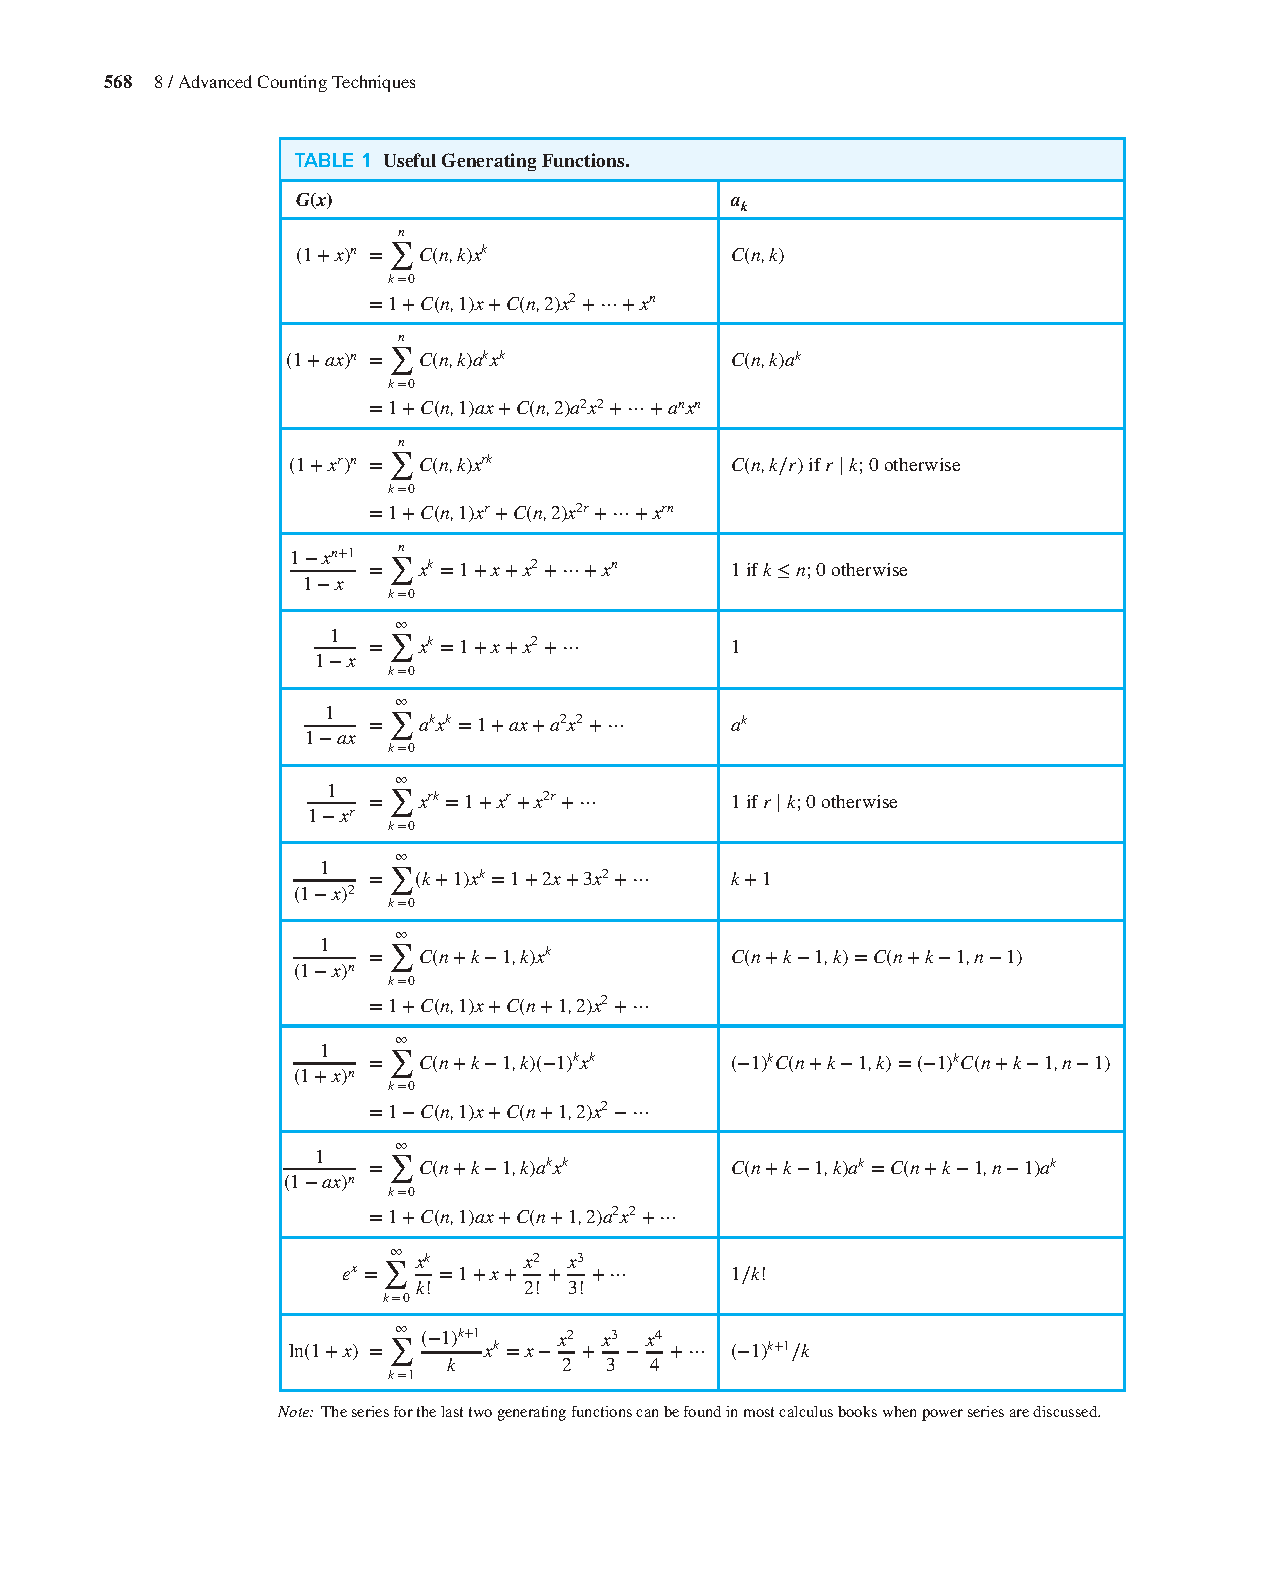
\includepdf[pages=-, width=\textwidth]{Useful-Generating-Functions.pdf}

\subsection{Counting Problems and Generating Functions}

Generating functions can be used to solve a wide variety of counting problems. In particular, they can be used to count the number of combinations of various types. We developed techniques to count the $r$-combinations from a set with n elements when repetition is allowed and additional constraints may exist. Such problems are equivalent to counting the solutions to equations of the form
\begin{equation*}
e_1 + e_2 + ... + e_n = C,    
\end{equation*}
where $C$ is a constant and each $e_i$ is a non-negative integer that may be subject to a specified constraint. Generating functions can also be used to solve counting problems of this type.

\begin{example}
Find the number of solutions of 
\begin{equation*}
    e_1 + e_2 + e_3 = 17,
\end{equation*}
where $e_1, e_2$ and $e_3$ are non-negative integers with $2 \leq e_1 \leq 5$, $3 \leq e_2 \leq 6$ and $4 \leq e_3 \leq 7$.

\textbf{Solution:}

The number of solutions with the indicated constraints is the coefficient of $x^{17}$ in the expansion of
\begin{equation*}
    (x^2 + x^3 + x^4 + x^5)(x^3 + x^4 + x^5 + x^6)(x^4 + x^5 + x^6 + x^7).
\end{equation*}
This follows because we obtain a term equal to $x^{17}$ in the product by picking a term in the first sum $x^{e_1}$, and a term in the third sum $x^{e_3}$, where the exponents $e_1, e_2$ and $e_3$ satisfy the equation $e_1 + e_2 + e_3 = 17$ and the given constraints. 

It is not hard to see that the coefficient of $x^{17}$ in this product is 3. Hence, there are three solutions.
\end{example}

\begin{example}
In how many different ways can eight identical cookies be distributed among three distinct children if each child receives at least two cookies and no more than four cookies?

\textbf{Solution:}

Because each child receives at least two but no more than four cookies, for each child there is a factor equal to
\begin{equation*}
    (x^2 + x^3 + x^4)
\end{equation*}
in the generating function for the sequence $\{c_n\}$, where $c_n$ is the number of ways to distribute $n$ cookies. Because there are three children, this generating function is
\begin{equation*}
    (x^2 + x^3 + x^4)^3
\end{equation*}
We need the coefficient of $x^8$ in this product. The reason is that the $x^8$ terms in the expansion correspond to the ways that three terms can be selected, with one from each factor, that have exponents adding up to 8. Furthermore, the exponents of the term from the first, second, and third factors are the numbers of cookies the first, second, and third children receive, respectively. Computation shows that this coefficient equals \textbf{6}. Hence, there are six ways to distribute the cookies so that each child receives at least two, but no more than four, cookies.
\end{example}

\subsection{Using Generating Functions to Solve Recurrence Relations}
We can find the solution to a recurrence relation and its initial conditions by finding an explicit formula for the associated generating function. This is illustrated in following examples.

\begin{example}
Solve the recurrence relation $a_k = 3a_{k-1}$ for $k = 1, 2, 3, ...$ and initial condition $a_0 = 2$.

\textbf{Solution:}

Let $G(x)$ be the generating function for the sequence $\{a_k\}$, that is, $G(x) = \sum_{k=0}^{\infty} a_kx^k$. First note that
\begin{equation*}
    x G(x) = \sum_{k=0}^{\infty} a_kx^{k+1} = \sum_{k=1}^{\infty} a_{k-1}x^k.
\end{equation*}
Using the recurrence relation, we see that
\begin{align*}
    G(x) - 3x G(x) &= \sum_{k=0}^{\infty} a_kx^k - 3 \sum_{k=1}^{\infty} a_{k-1}x^k\\
    &= a_0 + \sum_{k=1}^{\infty} (a_k - 3 a_{k-1})x^k\\
    &= 2,
\end{align*}
because $a_0 = 2$ and $a_k = 3a_{k-1}$. Thus,
\begin{equation*}
    G(x) - 3xG(x) = (1-3x)G(x) = 2
\end{equation*}
Solving for $G(x)$ shows that $G(x) = 2/(1-3x)$. Using the identity $1/(1-ax) = \sum_{k=0}^{\infty} a^kx^k$, from Table 1, we have
\begin{equation*}
    G(x) = 2 \sum_{k=0}^{\infty} 3^kx^k = \sum_{k=0}^{\infty} 2 \cdot 3^kx^k.
\end{equation*}
Consequently, $a_k = 2 \cdot 3^k$.
\end{example}


\newpage
\begin{example}
Suppose that a valid code-word is an $n$-digit number in decimal notation containing an even number of 0s. Let $a_n$ denote the number of valid code-words of length $n$. (In book, in Example 4 of Section
8.1, it is showed that the sequence $\{a_n\}$ satisfies the recurrence relation
\begin{equation*}
    a_nx^n = 8 a_{n-1}x^n + 10^{n-1}x^n
\end{equation*}
and the initial condition $a_1 = 9$. Use generating functions to find an explicit formula for $a_n$.

\textbf{Solution}

To make our work with generating functions simpler, we extend this sequence by setting $a_0 = 1$; when we assign this value to $a_0$ and use the recurrence relation, we have $a_1 = 8a_0 + 10^0 = 8 + 1 = 9$, which is consistent with our original initial condition. (It also makes sense bacuse there is one code-word of length 0 -the empty string.)

We multiply both sides of the recurrence relation by $x^n$ to obtain
\begin{equation*}
    a_nx^n = 8 a_{n-1}x^n + 10^{n-1}x^n
\end{equation*}
Let $G(x) = \sum_{k=0}^{\infty} a_nx^n$ be the generating function of the sequence $a_0, a_1, a_2, ...$. We sum both sides of the last equation starting with $n = 1$, to find that
\begin{align*}
    G(x) -1 &= \sum_{n=1}^{\infty} a_nx^n = \sum_{n=1}^{\infty} (8a_{n-1}x^n + 10^{n-1}x^n)\\
    &= 8 \sum_{n=1}^{\infty} a_{n-1}x^n + \sum_{n=1}^{\infty} 10^{n-1}x^n\\
    &= 8x \sum_{n=1}^{\infty} a_{n-1}x^{n-1} + x \sum_{n=1}^{\infty} 10^{n-1}x^{n-1}\\
    &= 8x \sum_{n=0}^{\infty} a_{n}x^{n} + x \sum_{n=0}^{\infty} 10^{n}x^{n}\\
    &= 8xG(x) + x/(1-10x),
\end{align*}
We have
\begin{equation*}
    G(x) - 1 = 8xG(x) + x/(1-10x)
\end{equation*}

Solving for $G(x)$ shows that
\begin{equation*}
    G(x) = \frac{1-9x}{(1-8x)(1-10x)}
\end{equation*}
Expanding the right-hand side of this equation into partial fractions (as is done in the integration of ratinoanl functions studied in calculus) gives
\begin{align*}
    G(x) &= \frac{1}{2} \left( \frac{1}{1-8x} + \frac{1}{1-10x} \right)\\
    G(x) &= \frac{1}{2} \left( \sum_{n=0}^{\infty} 8^nx^n + \sum_{n=0}^{\infty} 10^nx^n \right)\\
    G(x) &= \sum_{n=0}^{\infty} \frac{1}{2} (8^n + 10^n) x^n
\end{align*}
Consequently, we have shown that
\begin{equation*}
    a_n = \frac{1}{2} (8^n + 10^n)
\end{equation*}
\end{example}


\section{Inclusion–Exclusion}

\subsection{Introduction}

A discrete mathematics class contains 30 women and 50 sophomores. How many students in the class are either women or sophomores? This question cannot be answered unless more information is provided. Adding the number of women in the class and the number of sophomores probably does not give the correct answer, because women sophomores are counted twice. This observation shows that the number of students in the class that are either sophomores or women is the sum of the number of women and the number of sophomores in the class minus the number of women sophomores. 

In this section we will generalize the ideas introduced in that section to solve problems that require us to count the number of elements in the union of more than two sets.

\subsection{The Principle of Inclusion–Exclusion}

How many elements are in the union of two finite sets? The number of elements in the union of the two sets $A$ and $B$ is the sum of the numbers of elements in the sets minus the number of elements in their intersection. That is,
\begin{align*}
    |A \cup B| = |A| + |B| - |A \cap B|
\end{align*}

\noindent The formula for the number of elements in the union of two sets is useful in counting problems.


We will now begin our development of a formula for the number of elements in the union of a finite number of sets. The formula we will develop is called the principle of \textbf{inclusion–exclusion}. For concreteness, before we consider unions of $n$ sets, where $n$ is any positive integer, we will derive a formula for the number of elements in the union of three sets $A$, $B$, and $C$. To construct this formula, we note that $|A| + |B| + |C|$ counts each element that is in exactly one of the three sets once, elements that are in exactly two of the sets twice, and elements in all three sets three times. This is illustrated in the first panel in Figure 2.

\begin{figure}[h!]
    \centering
    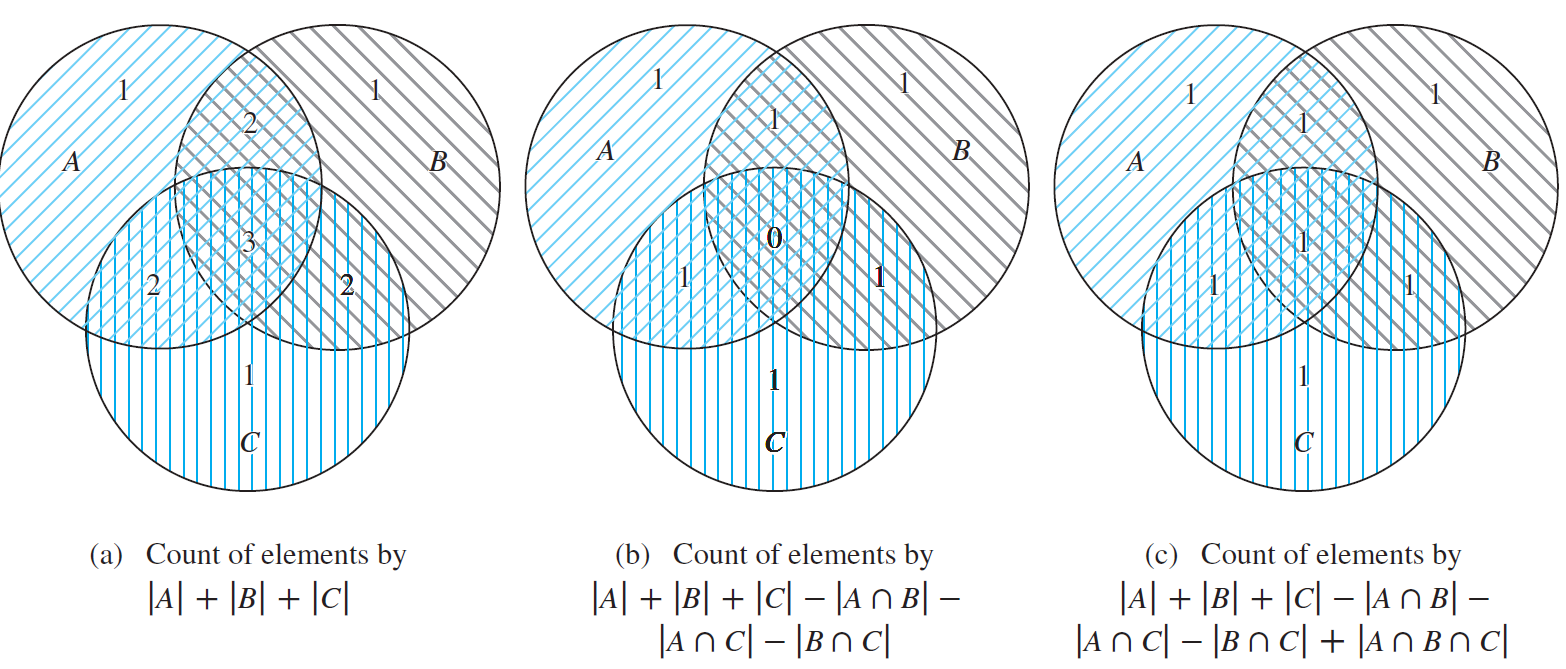
\includegraphics[width=.7\textwidth]{img/ch8.5-figure3.png}
    \caption{Finding a formula for the number of elements in the union of three sets.}
    \label{fig:my_label}
\end{figure}

To remove the overcount of elements in more than one of the sets, we subtract the number of elements in the intersections of all pairs of the three sets. We obtain
\begin{align*}
    |A| + |B| + |C| - |A \cap B| - |A \cap C| - |B \cap C|
\end{align*}

\noindent This expression still counts elements that occur in exactly one of the sets once. An element that occurs in exactly two of the sets is also counted exactly once, because this element will occur in one of the three intersections of sets taken two at a time. However, those elements that occur in all three sets will be counted zero times by this expression, because they occur in all three intersections of sets taken two at a time. This is illustrated in the second panel in Figure 3.

To remedy this undercount, we add the number of elements in the intersection of all three sets. This final expression counts each element once, whether it is in one, two, or three of the sets. Thus,
\begin{align*}
    |A \cup B \cup C| = |A| + |B| + |C| - |A \cap B| - |A \cap C| - |B \cap C| + |A \cap B \cap C|
\end{align*}

\noindent This formula is illustrated in the third panel of Figure 3.

We will now state and prove the \textbf{inclusion–exclusion principle} for $n$ sets, where $n$ is a positive integer. This principle tells us that we can count the elements in a union of $n$ sets by adding the number of elements in the sets, then subtracting the sum of the number of elements in all intersections of two of these sets, then adding the number of elements in all intersections of three of these sets, and so on, until we reach the number of elements in the intersection of all the sets. It is added when there is an odd number of sets and added when there is an even number of sets.

\begin{theorem}
{1}
\textbf{The Principle of Inclusion-Exclusion}

Let $A_1, A_2, ..., A_n$ be finite sets. Then



\begin{align*}
    |A_1 \cup A_2 \cup \cdots \cup A_n| &= \sum_{1 \leq i \leq n} |A_i| - \sum_{1 \leq i \leq j \leq n} |A_i \cap A_j|\\
    &+ \sum_{1 \leq i \leq j \leq k \leq n} |A_i \cap A_j \cap A_k| - \cdots + (-1)^{n+1} |A_1 \cap A_2 \cap \cdots \cap A_n|
\end{align*}
\end{theorem}

\textit{(Proof of the The Principle of Inclusion-Exclusion theorem should be read from textbook, page 583)}.


\begin{example}
Give a formula for the number of elements in the union of four sets.

\textbf{Solution:}
The inclusion–exclusion principle shows that
\begin{align*}
    |A_1 \cup A_2 \cup A_3 \cup A_4| &= |A_1| + |A_2| + |A_3| + |A_4|\\
    &- |A_1 \cap A_2| - |A_1 \cap A_3| - |A_1 \cap A_4| - |A_2 \cap A_3| - |A_2 \cap A_4| - |A_3 \cap A_4|\\
    &+ |A_1 \cap A_2 \cap A_3| + |A_1 \cap A_2 \cap A_4| + |A_1 \cap A_3 \cap A_4| + |A_2 \cap A_3 \cap A_4|\\
    &- |A_1 \cap A_2 \cap A_3 \cap A_4|.
\end{align*}

Note that this formula contains 15 different terms, one for each nonempty subset of $\{A_1, A_2, A_3, A_4\}$.
\end{example}

\section{Applications of Inclusion-Exclusion}

\subsection{Introduction}

Many counting problems can be solved using the principle of inclusion–exclusion. For instance, we can use this principle to find the number of primes less than a positive integer. Many problems can be solved by counting the number of onto functions from one finite set to another. The inclusion–exclusion principle can be used to find the number of such functions. The well-known hatcheck problem can be solved using the principle of inclusion–exclusion. This problem asks for the probability that no person is given the correct hat back by a hatcheck person who gives the hats back randomly.

\subsection{An Alternative Form of Inclusion–Exclusion}

There is an alternative form of the principle of inclusion–exclusion that is useful in counting problems. In particular, this form can be used to solve problems that ask for the number of elements in a set that have none of $n$ properties $P_1, P_2, ..., P_n$.

Let $A_i$ be the subset containing the elements that have property $P_i$. The number of elements with all the properties $P_{i_1}, P_{i_2}, ..., P_{i_k}$ will be denoted by $N(P_{i_1} P_{i_2} \cdots P_{i_k})$. Writing these quantities in terms of sets, we have
\begin{align*}
    &|A_{i_1} \cap A_{i_2} \cap \cdot \cdot \cdot \cap A_{i_k}| = N(P_{i_1} P_{i_2} \cdots P_{i_k}) & & & & & & & & & &
\end{align*}

\noindent If the number of elements with none of the properties $P_1, P_2, ..., P_n$. is denoted by $N(P_{i_1}^{'} P_{i_2}^{'} \cdots P_{i_k}^{'})$ and the number of elements in the set is denoted by $N$, it follows that
\begin{align*}
    &N(P_{1}^{'} P_{2}^{'} \cdots P_{n}^{'}) = N - |A_1 \cup A_2 \cup \cdot \cdot \cdot \cup A_n| & & & & & & & & & &
\end{align*}

\noindent From the inclusion–exclusion principle, we see that
\begin{align*}
    N(P_{1}^{'} P_{2}^{'} \cdots P_{n}^{'}) &= N - \sum_{1 \leq i \leq n} N(P_i) + \sum_{1 \leq i \leq j \leq n} N(P_iP_j)\\
    &=-\sum_{1 \leq i \leq j \leq k \leq n} N(p_iP_jP_k) + \cdot \cdot \cdot + (-1)^n N(P_1P_2 \cdots P_n)
\end{align*}

The following example shows how the principle of inclusion–exclusion can be used to determine the number of solutions in integers of an equation with constraints.

\begin{example}
How many solutions does
\begin{align*}
    x_1 + x_2 + x_3 = 11 &&&&&&&&&&&&&&&&&
\end{align*}
have, where $x_1$, $x_2$, and $x_3$ are nonnegative integers with $x_1 \leq 3$, $x_2 \leq 4$, and $x_3 \leq 6$?

\textbf{Solution:}
To apply the principle of inclusion–exclusion, let a solution have property $P_1$ if $x_1 > 3$, property $P_2$ if $x_2 > 4$, and property $P_3$ if $x_3 > 6$. The number of solutions satisfying the inequalities $x_1 \leq 3$, $x_2 \leq 4$, and $x_3 \leq 6$ is 
\begin{align*}
    N(P_1^{'}P_2^{'}P_3^{'}) = N - N(P_1) - N(P_2) - N(P_3) + N(P_1P_2) N(P_1P_3) + N(P_2P_3) - N(P_1P_2P_3)
\end{align*}
\\
\begin{itemize}
    \item $N$ = total number of solutions = $C(3 + 11 - 1, 11) = 78$,
    \item $N(P_1)$ = (number of solutions with $x_1 \geq 4$) = $C(3 + 7 - 1, 7) = C(9, 7) = 36$,
    \item $N(P_2)$ = (number of solutions with $x_2 \geq 5$) = $C(3 + 6 - 1, 6) = C(8, 6) = 28$,
    \item $N(P_3)$ = (number of solutions with $x_3 \geq 7$) = $C(3 + 4 - 1, 4) = C(6, 4) = 15$,
    \item $N(P_1P_2)$ = (number of solutions with $x_1 \geq 4$ and $x_2 \geq 5$) = $C(3 + 2 - 1, 2) = C(4, 2) = 6$,
    \item $N(P_1P_3)$ = (number of solutions with $x_1 \geq 4$ and $x_3 \geq 7$) = $C(3 + 0 - 1, 0) = 1$,
    \item $N(P_2P_3)$ = (number of solutions with $x_2 \geq 5$ and $x_3 \geq 7$) = $0$,
    \item $N(P_1P_2P_3)$ = (number of solutions with $x_1 \geq 4$, $x_2 \geq 5$, and $x_3 \geq 7$) = $0$.
\end{itemize}

Inserting these quantities into the formula for $N(P_1^{'}P^{'}_2P^{'}_3)$ shows that the number of solutions with $x_1 \leq 3$, $x_2 \leq 4$, and $x_3 \leq 6$ equals 
\begin{align*}
    N(P_1^{'}P^{'}_2P^{'}_3) = 78 - 36 - 28 - 15 + 6 + 1 + 0 - 0 = 6
\end{align*}
\end{example}

\subsection{The Sieve of Eratosthenes}

Because the only primes not exceeding 10 (by algorithm, $\sqrt{100}$) are 2, 3, 5, and 7, the primes not exceeding 100 are these four primes and those positive integers greater than 1 and not exceeding 100 that are divisible by \textit{none} of 2, 3, 5, or 7. To apply the principle of inclusion–exclusion, let $P_1$ be the property that an integer is divisible by 2, let $P_2$ be the property that an integer is divisible by 3, let $P_3$ be the property that an integer is divisible by 5, and let $P_4$ be the property that an integer is divisible by 7. Thus, the number of primes not exceeding 100 is
\begin{align*}
    4 + N(P_1^{'}P_2^{'}P_3^{'}P_4^{'})&&&&&&&&&&&&&
\end{align*}
Because there are 99 positive integers greater than 1 and not exceeding 100, the principle of inclusion–exclusion shows that
\begin{align*}
    N(P_1^{'}P_2^{'}P_3^{'}P_4^{'}) &= 99 - N(P_1) - N(P_2) - N(P_3) - N(P_4)\\
    &+ N(P_1P_2) + N(P_1P_3) + N(P_1P_4) + N(P_2P_3) + N(P_2P_4) + N(P_3P_4)\\
    &- N(P_1P_2P_3) - N(P_1P_2P_4) - N(P_1P_3P_4) - N(P_2P_3P_4)\\
    &+ N(P_1P_2P_3P_4)
\end{align*}
The number of integers not exceeding 100 (and greater than 1) that are divisible by all the primes in a subset of $\{2, 3, 5, 7\}$ is $\lfloor 100/N \rfloor$, where $N$ is the product of the primes in this subset. (This follows because any two of these primes have no common factor.) Consequently,

\begin{align*}
    N(P_1^{'}P_2^{'}P_3^{'}P_4^{'}) &= 99 - \left\lfloor\dfrac{100}{2}\right\rfloor - \left\lfloor\dfrac{100}{3}\right\rfloor - \left\lfloor\dfrac{100}{5}\right\rfloor - \left\lfloor\dfrac{100}{7}\right\rfloor\\
    &+ \left\lfloor\dfrac{100}{2\cdot3}\right\rfloor + \left\lfloor\dfrac{100}{2\cdot5}\right\rfloor + \left\lfloor\dfrac{100}{2\cdot7}\right\rfloor + \left\lfloor\dfrac{100}{3\cdot5}\right\rfloor + 
    \left\lfloor\dfrac{100}{3\cdot7}\right\rfloor + \left\lfloor\dfrac{100}{5\cdot7}\right\rfloor\\
    &- \left\lfloor\dfrac{100}{2\cdot3\cdot5}\right\rfloor - \left\lfloor\dfrac{100}{2\cdot3\cdot7}\right\rfloor - \left\lfloor\dfrac{100}{2\cdot5\cdot7}\right\rfloor - \left\lfloor\dfrac{100}{3\cdot5\cdot7}\right\rfloor + \left\lfloor\dfrac{100}{2\cdot3\cdot5\cdot7}\right\rfloor\\
    &= 99 - 50 - 33 - 20 - 14 + 16 + 10 + 7 + 6 + 4 + 2 - 3 - 2 - 1 - 0 + 0\\
    &= 21
\end{align*}
Hence, there are 4 + 21 = 25 primes not exceeding 100.

\subsection{The Number of Onto Functions}

The principle of inclusion–exclusion can also be used to determine the number of onto functions from a set with $m$ elements to a set with $n$ elements.

\begin{example}
How many onto functions are there from a set with six elements to a set with three elements?

\textbf{Solution:}
Suppose that the elements in the codomain are $b_1$, $b_2$, and $b_3$. Let $P_1$, $P_2$, and $P_3$ be the properties that $b_1$, $b_2$, and $b_3$ are not in the range of the function, respectively. Note that a function is onto if and only if it has none of the properties $P_1$, $P_2$, or $P_3$. By the inclusion– exclusion principle it follows that the number of onto functions from a set with six elements to a set with three elements is 
\begin{align*}
    N(P_1^{'} P_2^{'} P_3^{'}) &= N - [N(P_1) + N(P_2) + N(P_3)]\\
    &+ [N(P_1P_2) + N(P_1P_3) + N(P_2P_3)] - N(P_1P_2P_3)
\end{align*}
where $N$ is the total number of functions from a set with six elements to one with three elements. We will evaluate each of the terms on the right-hand side of this equation.

$N = 3^6$. Note that $N(P_i)$ is the number of functions that do not have $b_i$ in their range. Hence, there are two choices for the value of the function at each element of the domain. Therefore, $N(P_i) = 2^6$. Furthermore, there are $C(3, 1)$ terms of this kind. Note that $N(P_iP_j)$ is the number of functions that do not have $b_i$ and $b_j$ in their range. Hence, there is only one choice for the value of the function at each element of the domain. Therefore, $N(P_iP_j) = 1^6 = 1$. Furthermore, there are $C(3, 2)$ terms of this kind. Also, note that $N(P_1P_2P_3) = 0$, because this term is the number of functions that have none of $b_1$, $b_2$, and $b_3$ in their range. Clearly, there are no such functions, so the number of onto functions from a set with six elements to one with three elements is 
\begin{align*}
    3^6 - C(3, 1) 2^6 + C(3, 2) 1^6 = 729 - 192 + 3 = 540&&&&&&
\end{align*}
\end{example}

\newpage
The general result that tells us how many onto functions there are from a set with $m$ elements to one with $n$ elements will now be stated.

\begin{theorem}
{1}
Let $m$ and $n$ be positive integers with $m \geq n$. Then, there are
\begin{align*}
    n^m - C(n, 1)(n - 1)^m + C(n, 2)(n - 2)^m - \cdot \cdot \cdot + (-1)^{n-1}C(n, n - 1) \cdot 1^m
\end{align*}
onto functions from a set with $m$ elements to a set with $n$ elements.
\end{theorem}

\section{Derangements}

The principle of inclusion–exclusion will be used to count the permutations of $n$ objects that leave no objects in their original positions. Consider the following example.

\begin{example}[The Hatcheck Problem]
A new employee checks the hats of $n$ people at a restaurant, forgetting to put claim check numbers on the hats. When customers return for their hats, the checker gives them back hats chosen at random from the remaining hats. What is the probability that no one receives the correct hat?
\end{example}

\textbf{Remark:} The answer is the number of ways the hats can be arranged so that there is no hat in its original position divided by $n!$, the number of permutations of $n$ hats. We will return to this example after we find the number of permutations of n objects that leave no objects in their original position.

A \textbf{derangement} is a permutation of objects that leaves no object in its original position. To solve the problem posed in the above example we will need to determine the number of \textit{derangements} of a set of $n$ objects.

\begin{example}
The permutation 21453 is a derangement of 12345 because no number is left in its original position. However, 21543 is not a derangement of 12345, because this permutation leaves 4 fixed.
\end{example}

Let $D_n$ denote the number of derangements of $n$ objects. For instance, $D_3 = 2$, because the derangements of 123 are 231 and 312. We will evaluate $D_n$, for all positive integers $n$, using the principle of inclusion–exclusion.

\begin{theorem}{2}
The number of derangements of a set with $n$ elements is
\begin{align*}
    D_n = n! \left[ 1 - \dfrac{1}{1!} + \dfrac{1}{2!} - \dfrac{1}{3!} + \cdot \cdot \cdot + (-1)^n \dfrac{1}{n!} \right]
\end{align*}
\end{theorem}

\textit{(The proof of the Theorem 2 should be read from book)}.

\newpage
It is now straightforward to find $D_n$ for a given positive integer $n$. For instance, using Theorem 2, it follows that
\begin{align*}
    D_3 = 3! \left[ 1 - \dfrac{1}{1!} + \dfrac{1}{2!} - \dfrac{1}{3!} \right] = 6 \left(1 - 1 + \dfrac{1}{2} - \dfrac{1}{6} \right) = 2
\end{align*}
as we have previously remarked.

The solution of "The Hatcheck Problem" can now be given

\begin{example}[The Hatcheck Problem]
\textbf{Solution:}
The probability that no one receives the correct hat is $D_n / n!$. By Theorem 2, this probability is
\begin{align*}
    \dfrac{D_n}{n!} = 1 - \dfrac{1}{1!} + \dfrac{1}{2!} - \cdot \cdot \cdot + (-1)^n \dfrac{1}{n!}
\end{align*}
\end{example}

By the identity $e^x = \sum_{j=0}^{\infty} x^j / j!$ for all real numbers $x$ (from calculus), we know that
\begin{align*}
    e^{-1} = 1 - \frac{1}{1!} + \frac{1}{2!} - \cdot \cdot \cdot (-1)^n \frac{1}{n!} \approx 0.368
\end{align*}
Because this is an alternating series with terms tending to zero, it follows that as $n$ grows without bound, the probability that no one receives the correct hat converges to $e^{-1} \approx 0.368$. In fact, this probability can be shown to be within $1/(n + 1)!$ of $e^{-1}$.


\newpage
\begin{center}
\section*{Key Terms and Results}
\end{center}

\begin{multicols}{2}

\begin{center}
    \textbf{TERMS}
\end{center}

\textbf{recurrence relation:} a formula expressing terms of a sequence, except for some initial terms, as a function of one or more previous terms of the sequence

\textbf{initial conditions for a recurrence relation:} the values of the terms of a sequence satisfying the recurrence relation before this relation takes effect

\textbf{dynamic programming:} an algorithmic paradigm that finds the solution to an optimization problem by recursively breaking down the problem into overlapping subproblems and combining their solutions with the help of a recurrence relation

\textbf{linear homogeneous recurrence relation with constant coefficients:} a recurrence relation that expresses the terms of a sequence, except initial terms, as a linear combination of previous terms

\textbf{characteristic roots of a linear homogeneous recurrence relation with constant coefficients:} the roots of the polynomial associated with a linear homogeneous recurrence relation with constant coefficients

\textbf{linear nonhomogeneous recurrence relation with constant coefficients:} a recurrence relation that expresses the terms of a sequence, except for initial terms, as a linear combination of previous terms plus a function that is not identically zero that depends only on the index

\textbf{divide-and-conquer algorithm:} an algorithm that solves a problem recursively by splitting it into a fixed number of smaller nonoverlapping subproblems of the same type

\textbf{generating function of a sequence:} the formal series that has the $n$th term of the sequence as the coefficient of $x_n$

\textbf{sieve of Eratosthenes:} a procedure for finding the primes less than a specified positive integer

\textbf{derangement:} a permutation of objects such that no object is in its original place

\begin{center}
\textbf{RESULTS}
\end{center}

\textbf{the formula for the number of elements in the union of two finite sets:}
\begin{equation*}
    |A \cup B| = |A| + |B| - |A \cap B|
\end{equation*}

\textbf{the formula for the number of elements in the union of three finite sets:}
\begin{align*}
    |A \cup B \cup C| &= |A| + |B| + |C|\\
    &- |A \cap B| - |A \cap C| - |B \cap C|\\
    &+ |A \cap B \cap C|
\end{align*}

\textbf{the principle of inclusion–exclusion:}
\begin{align*}
    |A_1 \cup A_2 \cup \cdots \cup A_n| &= \sum_{1 \leq i \leq n} |A_i| - \sum_{1 \leq i \leq j \leq n} |A_i \cap A_j|\\
    &+ \sum_{1 \leq i \leq j \leq k \leq n} |A_i \cap A_j \cap A_k|\\
    &- \cdots + (-1)^{n+1} |A_1 \cap A_2 \cap \cdots \cap A_n|
\end{align*}

\textbf{the number of onto functions from a set with $m$ elements to a set with $n$ elements:}
\begin{align*}
    n^m - C(n, 1)(n - 1)^m &+ C(n, 2)(n - 2)^m\\
    &- \cdot \cdot \cdot + (-1)^{n-1}C(n, n - 1) \cdot 1^m
\end{align*}

\textbf{the number of derangements of $n$ objects:}
\begin{align*}
    D_n = n! \left[ 1 - \dfrac{1}{1!} + \dfrac{1}{2!} - \dfrac{1}{3!} + \cdot \cdot \cdot + (-1)^n \dfrac{1}{n!} \right]
\end{align*}
\end{multicols}


\end{document}
